\chapter*{Zoznam príloh}
\addcontentsline{toc}{chapter}{Zoznam príloh}

\begin{description}[leftmargin=3cm, labelsep=0.5cm]
    \item[Príloha 1] Žiadosť o povolenie výskumu
    \item[Príloha 2] Vlastný dotazník
\end{description}

\clearpage

\vspace*{7cm}
\begin{center}
    \Huge\textbf{PRÍLOHY}
\end{center}
\thispagestyle{empty}
\clearpage

\section*{Príloha 1 Žiadosť o povolenie výskumu}
\addcontentsline{toc}{section}{Príloha 1 Žiadosť o povolenie výskumu}

\vspace{1cm}
\begin{flushright}
    Bc. Roman Ballek\\
    študent 2. ročníka Mgr. štúdia\\
    Fakulta zdravotníctva TnUAD
\end{flushright}

\vspace{1cm}
\noindent Vec: \textbf{Žiadosť o povolenie vykonania výskumu pre účely diplomovej práce}

\vspace{1cm}
\noindent Vážený pán riaditeľ / Vážená pani riaditeľka,

\vspace{0.5cm}
\noindent týmto Vás zdvorilo žiadam o povolenie vykonania výskumu v~priestoroch Vášho zdravotníckeho zariadenia. Výskum je realizovaný v~rámci mojej diplomovej práce na tému \textbf{„\nazovprace“} pod odborným vedením \veduci.

\vspace{0.5cm}
\noindent Výskum je anonymný a~získané údaje budú použité výhradne na vedecké účely a~spracovanie mojej záverečnej práce. Súčasťou výskumu je goniometrické meranie postihnutých kĺbov a~vypĺňanie dotazníka zameraného na kvalitu života pacientov s~reumatoidným ochorením.

\vspace{0.5cm}
\noindent Za kladné vybavenie mojej žiadosti Vám vopred ďakujem.

\vspace{1.5cm}
\noindent V~Trenčíne dňa \dots\dots\dots\dots\dots\dots \hfill \dots\dots\dots\dots\dots\dots\dots\dots\dots\\
\hspace*{9.5cm} Podpis študenta

\clearpage

\section*{Príloha 2 Vlastný dotazník}
\addcontentsline{toc}{section}{Príloha 2 Vlastný dotazník}

\begin{center}
    \textbf{Dotazník}
\end{center}

\noindent Vážený respondent/respondentka, obdržali ste anonymný dotazník, ktorý slúži len pre potreby spracovania diplomovej práce na tému \textit{Využitie fyzioterapie u~pacientov s~reumatickým ochorením} na Trenčianskej univerzite Alexandra Dubčeka v~Trenčíne.

\noindent Prosíme vás, aby ste pri vypĺňaní zvolili najpravdivejšie možné odpovede. Ak nie ste istí správnou odpoveďou, vyberte možnosť, ktorá najlepšie zodpovedá vašej situácii. V~otázkach je možné označiť len 1 odpoveď. Všetky otázky sú povinné.

\noindent Vopred Vám ďakujeme za vyplnenie Bc. Roman Ballek.

\vspace{0.5cm}
\noindent \textbf{Demografické údaje:}

\noindent Pohlavie : \dots\dots\dots\dots\dots\dots \\
Vek: \dots\dots\dots\dots\dots\dots rokov \\
Výška : \dots\dots\dots\dots\dots\dots cm \\
Hmotnosť : \dots\dots\dots\dots\dots\dots kg

\vspace{0.5cm}
\noindent 1. Zamestnanie / Typ zaťaženia:
\begin{enumerate}[label=\arabic*.]
    \item aktívne
    \item sedavé
    \item nezamestnaný / dôchodca
\end{enumerate}

\noindent 2. Subjektívne hodnotenie stupňa bolesti pred začatím liečby (zakrúžkujte):

\noindent (žiadna bolesť) \hfill (neznesiteľná bolesť)
\begin{center}
    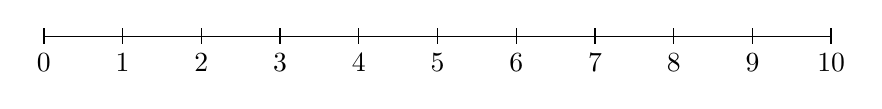
\begin{tikzpicture}
        \draw[|-|] (0,0) -- (10,0);
        \foreach \x in {0,1,2,3,4,5,6,7,8,9,10}
            \draw (\x,0.1) -- (\x,-0.1) node[below] {\x};
    \end{tikzpicture}
\end{center}

\noindent 3. Typ bolesti:
\begin{enumerate}[label=\arabic*.]
    \item tupá
    \item pálivá
    \item bodavá
    \item pulzujúca
    \item tlaková
\end{enumerate}

\noindent 4. Zakrúžkujte čas najsilnejšej bolesti počas dňa:
\begin{center}
    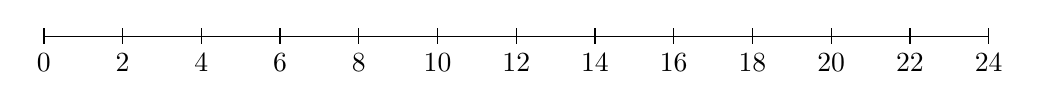
\begin{tikzpicture}
        \draw[|-|] (0,0) -- (12,0);
        \foreach \x [evaluate=\x as \label using int(\x*2)] in {0,1,2,3,4,5,6,7,8,9,10,11,12}
            \draw (\x,0.1) -- (\x,-0.1) node[below] {\label};
    \end{tikzpicture}
\end{center}

\noindent 5. Ranná stuhnutosť:
\begin{enumerate}[label=\arabic*.]
    \item áno
    \item nie
\end{enumerate}

\vspace{0.3cm}
\noindent 6. Ohodnoťte vplyv ochorenia na nasledujúce oblasti (0 - žiadne, 10 - neznesiteľné/úplná neschopnosť):

\begin{table}[H]
\centering
\begin{tabular}{p{8cm} c}
ADL (obliekanie, hygiena, stravovanie): & \dots\dots\dots \\
Bolesť v kľude: & \dots\dots\dots \\
Bolesť pri záťaži: & \dots\dots\dots \\
Bolesť v zápästí: & \dots\dots\dots \\
Bolesť v kĺboch ruky (MCP, PIP): & \dots\dots\dots \\
Bolesť v kĺboch nohy (MTP): & \dots\dots\dots \\
Intenzita rannej stuhnutosti: & \dots\dots\dots \\
Únava počas dňa: & \dots\dots\dots \\
Jemná motorika (zapínanie, úchop): & \dots\dots\dots \\
Kvalita spánku / Psychosociálne aspekty: & \dots\dots\dots \\
\end{tabular}
\end{table}

\noindent 7. Dynamické testy kĺbov (vypĺňa fyzioterapeut):

\begin{table}[H]
\centering
\begin{tabular}{|p{4.5cm}|c|c|c|c|}
\hline
\multirow{2}{*}{\textbf{Sledovaný kĺb}} & \multicolumn{2}{c|}{\textbf{Pred terapiou (cm/$^\circ$)}} & \multicolumn{2}{c|}{\textbf{Po terapii (cm/$^\circ$)}} \\ \hhline{~----}
 & \textbf{Dx} & \textbf{Sin} & \textbf{Dx} & \textbf{Sin} \\ \hline
Zápästný kĺb (flexia) & & & & \\ \hline
Zápästný kĺb (extenzia) & & & & \\ \hline
MCP kĺby (flexia) & & & & \\ \hline
MCP kĺby (extenzia) & & & & \\ \hline
PIP kĺby (flexia) & & & & \\ \hline
MTP kĺby (flexia) & & & & \\ \hline
MTP kĺby (extenzia) & & & & \\ \hline
\end{tabular}
\end{table}

\noindent 8. Subjektívne hodnotenie stupňa bolesti po ukončení liečby (zakrúžkujte):

\noindent (žiadna bolesť) \hfill (neznesiteľná bolesť)
\begin{center}
    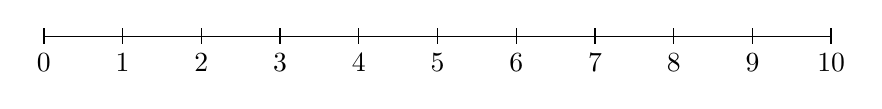
\begin{tikzpicture}
        \draw[|-|] (0,0) -- (10,0);
        \foreach \x in {0,1,2,3,4,5,6,7,8,9,10}
            \draw (\x,0.1) -- (\x,-0.1) node[below] {\x};
    \end{tikzpicture}
\end{center}

\clearpage
